\title{Study Guide for Midterm 1 for Algebra-Based Physics-2: Electricity, Magnetism, and Modern Physics (PHYS135B-01)}
\author{Dr. Jordan Hanson - Whittier College Dept. of Physics and Astronomy}
\date{\today}
\documentclass[10pt]{article}
\usepackage[a4paper, total={18cm, 27cm}]{geometry}
\usepackage{outlines}
\usepackage[sfdefault]{FiraSans}
\usepackage{hyperref}
\usepackage{graphicx}
\begin{document}
\maketitle

\begin{enumerate}
\item \textbf{Applications of circuits, Chapter 21}:
\begin{enumerate}
\item A 1000 W toaster and a 1000 W microwave are connected to the 120 V outlet.  Will this blow the 15 A fuse? \textbf{Yes.  Use $P = iV$ to find the current of $50/3$ amps.}
\item What is the total resistance of the system?  What is the resistance of each device? \textbf{The total resistance is given by Ohm's law: $V = i R$.  From the first part, $i = 50/3$ amps, and $V = 120$ V.  Thus, $R = (36/5) \Omega$.  Because each device consumes equal power, each must have equal resistance.  For two resistors connected in parallel, $R_{tot} = R/2$, where $R$ is the resistance of each device.  So $R = 2 R_{tot} = 36/5 \times 2 \Omega = 72/5 \Omega $.}
\item If the toaster were disconnected, what would be the total current? \textbf{The current should decrease by half, so $i = 25/3$ amps.}
\item What is highest wattage that could be connected to the wall with the microwave that would not blow the 15 A fuse? \textbf{Do the algebra: $P + x = iV$ and solve for $x$ when $P = 1000$ W, $i = 15$ amps, and $V = 120$ V.  It turns out to be: $x = iV - P = 15*120 - 1000 = 800$ W.}
\end{enumerate}
\item \textbf{Magnetism, Chapter 22}:
\begin{enumerate}
\item Draw the magnetic field of the Earth, and mark the location of the magnetic south and north poles on the Earth.  Estimate the angle of the Earth's magnetic field with respect to the ground in California, and at the South Pole. \textbf{The correct picture is shown in the text on p. 866 (Figure 22.23).  California is at 34 degrees N, meaning the field points partially \textit{down} and partially \textbf{North}.  At the equator the field is horizontal, and at the north pole it is straight down.}
\item What are the signs of the charged particles in Fig \ref{fig:magfield}? \textbf{The left particle is positive, the middle particle is neutral, and the right particle is negative.}
\begin{figure}[ht]
\centering
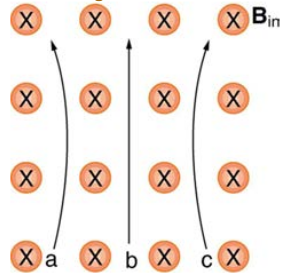
\includegraphics[width=0.2\textwidth]{magfield.png}
\caption{\label{fig:magfield} A magnetic field into the page with three potentially charged particles passing through it.}
\end{figure}
\item If the B-field in Fig. \ref{fig:magfield} has a strength of 0.001 T, and the particles at left and right are moving in circular paths with radius 1.0 m, what is the speed of these particles? \textbf{The centripedal force is provided by the magnetic force.  $qvB = mv^2/r \rightarrow v = (q/m) B r$.  Suppose the mass is that of a proton: $10^{-30}$ kg.  Then we have $1.6 \times 10^{-19} / 10^{-30} 10^{-3} 1.0 = 1.6 \times 10^8$ m/s.  This is less than the speed of light, so it's a reasonable result.}
\end{enumerate}
\item \textbf{Magnetism 2, Chapter 23}:
\begin{enumerate}
\item Recall that the definition of magnetic flux through an area $A$ by a B-field $B$ is $\phi = \vec{B} \cdot \vec{A} = BA\cos\theta$. See Fig 2.  What is the flux of a 0.001 T B-field passing through an area of 10 cm$^2$ at a 45 degree angle? \textbf{This is a plug-and-chug situation.  If one wants to convert units, remember that 1 cm$^2$ = $10^{-4}$ m$^2$.}
\item Let a solenoid shaped wire have $N$ coils, and let $\Delta \phi$ be the change in flux through the cross-sectional area $A$ of the coils.  Let $\Delta t$ be the change in time.  Recall that Faraday's law for coils of wire states that $emf = -N \Delta \phi/\Delta t$.  Suppose $A = 10$ cm$^2$, and $N = 1000$.  If a +0.001 T magnet moves through the coils in 1 ms, what voltage do we predict to \textit{appear} in the wire, from Faraday's Law?  Pay attention to the signs. \textbf{We have to derive the flux: $\phi = BA = 10^{-3} 10^{-3}$ T m$^2$.  Then we divide by 1 millisecond = $10^{-3}$ seconds, multiply by $N = 1000$, and don't forget the minus sign.  The result is -1 T m$^2$ s$^{-1}$, which is -1 V.}
\end{enumerate}
\end{enumerate}
\end{document}